% -*- Mode:TeX -*-

%% The documentclass options along with the pagestyle can be used to generate
%% a technical report, a draft copy, or a regular thesis.  You may need to
%% re-specify the pagestyle after you \include  cover.tex.  For more
%% information, see the first few lines of mitthesis.cls.

%\documentclass[12pt,vi,twoside]{mitthesis}
%%
%%  If you want your thesis copyright to you instead of MIT, use the
%%  ``vi'' option, as above.
%%
%\documentclass[12pt,twoside,leftblank]{mitthesis}
%%
%% If you want blank pages before new chapters to be labelled ``This
%% Page Intentionally Left Blank'', use the ``leftblank'' option, as
%% above.

% \documentclass[12pt,twoside]{mitthesis}

\documentclass[12pt]{article}

%% dsm: Place new refs last
\usepackage[hyphens]{url}

\usepackage{siunitx}
\usepackage{verbatim}
\usepackage{graphicx,afterpage}
\usepackage{yfonts}
%\usepackage{amsmath}
\usepackage{mathtools}
\usepackage{stmaryrd}
%\usepackage{amsfonts}
\usepackage{calc}
\usepackage{xspace}
\usepackage{listings}
\usepackage{multirow, booktabs}
\usepackage{wrapfig}
\usepackage{enumitem}
\usepackage{caption}
% \usepackage[labelformat=simple]{subcaption}
\usepackage{dblfloatfix} % to allow two-column floats at the bottom of the page
\usepackage{fixltx2e}
\usepackage{fancyhdr}
\usepackage{paralist}
\usepackage{color}


% https://tex.stackexchange.com/questions/240141/
\usepackage[T1]{fontenc} % Avoid garbling symbols and accents

\usepackage[keeplastbox]{flushend}




%For fancy tables
\usepackage{array} % decent table formatting
\usepackage{rotating}

\begin{comment}

\newcommand{\zzzNoOpSortToEnd}{}

% \usepackage[activate={true,nocompatibility},final,tracking=false,kerning=true,spacing=true]{microtype}
\setdefaultleftmargin{1.3em}{2em}{}{}{}{}

% asf: stole this from HATS
\lstdefinestyle{custompython}{ %aboveskip=0in,
 basewidth=0.5em,
 belowskip=0in,
 belowcaptionskip=-10pt,
 breaklines=true,
 captionpos=b,
 language=Python,
 showstringspaces=false,
 numbers=left,
 stepnumber=1,
 % dsm: semibold
 basicstyle={\linespread{0.9}\fontseries{sb}\small\ttfamily},
 keywordstyle=\bfseries,
 xleftmargin=2em,
 frame=single,
 framexleftmargin=2em,
 commentstyle=\itshape\color{green!40!black},
 morekeywords={to,yield},
}


% from figures.pptx
\definecolor{ltred}{HTML}{FB9A99}
\definecolor{dkred}{HTML}{E41A1C}
\definecolor{dkorange}{HTML}{F07F03}
\definecolor{ltorange}{HTML}{F7C090}
\definecolor{dkgreen}{HTML}{3BA32F}
\definecolor{ltgreen}{HTML}{B2E089}
\definecolor{dkblue}{HTML}{2879B4}
\definecolor{ltblue}{HTML}{A6CEE2}
\definecolor{dkpurple}{HTML}{6A3D9A}
\definecolor{ltpurple}{HTML}{CAB1D7}


% Spacing
\setlength{\textfloatsep}{8pt}
\setlist[enumerate]{leftmargin=0.25in,itemsep=1pt,topsep=1pt}

% More compact paragraphs
\makeatletter
\renewcommand{\paragraph}[1]{\noindent {\bf #1}}
\makeatother

\newcommand{\topbanner}{\textbf{DRAFT --- \input{auto_header.tex}}}
%\newcommand{\topbanner}{\textsc{Under Submission --- Please Do Not Distribute}}


% dsm: Fix citation format
\makeatletter
\def\citepunct{, }
\def\citedash{--}
\makeatother

% submission/web version
%\pagenumbering{arabic}

\captionsetup[figure]{aboveskip=2pt,belowskip=-12pt}

% If you comment hyperref and then uncomment it, make clean first (or kill .aux files)
\definecolor{lcolor}{RGB}{0, 56, 186} % {0, 35, 102}


\def\figureautorefname{Fig.}
\def\subfigureautorefname{Fig.}
\def\sectionautorefname{Sec.}
\def\subsectionautorefname{Sec.}
\def\algorithmautorefname{Algorithm\xspace}
\def\paragraphautorefname{Sec.}
\def\equationautorefname{Eq.}

% Temporary macros. Comment for submission!
% \newcommand{\note}[1]{{\bf [~NOTE:~#1~]}}
% \newcommand{\fixme}[1]{{\textcolor{red}{{\bf [~FIXME:~#1~]}}}}
% \newcommand{\todo}[1]{\textcolor{red}{{\bf [~TODO:~#1~]}}}
% \newcommand{\tmp}[1]{{\textcolor{red}{#1}}}
% \newcommand{\OK}[1]{{#1}}

\renewcommand*{\ttdefault}{txtt}

\renewcommand{\iscasubmissionnumber}{194}

%dsm: all these are retweaked
% Alter some LaTeX defaults for better treatment of figures:
% See p.105 of "TeX Unbound" for suggested values.
% See pp. 199-200 of Lamport's "LaTeX" book for details.
%   General parameters, for ALL pages:
\renewcommand{\topfraction}{0.9}        % max fraction of floats at top
\renewcommand{\bottomfraction}{0.8}     % max fraction of floats at bottom
%   Parameters for TEXT pages (not float pages):
\setcounter{topnumber}{5}
\setcounter{bottomnumber}{5}
\setcounter{totalnumber}{4}     % 2 may work better
\setcounter{dbltopnumber}{5}    % for 2-column pages
\renewcommand{\dbltopfraction}{0.9}     % fit big float above 2-col. text
\renewcommand{\textfraction}{0.07}      % allow minimal text w. figs
%   Parameters for FLOAT pages (not text pages):
\renewcommand{\floatpagefraction}{0.9}  % require fuller float pages
% N.B.: floatpagefraction MUST be less than topfraction !!
\renewcommand{\dblfloatpagefraction}{0.9}       % require fuller float pages

\definecolor{tableaublue}{rgb}{0.44,0.62,0.81}
\definecolor{tableauorange}{rgb}{0.9,0.55,0.25} % original tableau value: {1.,0.62,0.29}
\definecolor{tableaugreen}{rgb}{0.4,0.75,0.36}
\definecolor{tableaured}{rgb}{0.93,0.4,0.36}
\definecolor{tableaupurple}{rgb}{0.68,0.55,0.79}
\newcommand{\green}[1]{\textcolor{tableaugreen}{\sf\bfseries #1}}
\newcommand{\orange}[1]{\textcolor{tableauorange}{\sf\bfseries #1}}
%\newcommand{\blue}[1]{\textcolor{tableaublue}{\sf\bfseries #1}}
\newcommand{\red}[1]{\textcolor{tableaured}{\sf\bfseries #1}}
%\newcommand{\purple}[1]{\textcolor{tableaupurple}{\sf\bfseries #1}}


\usepackage{pifont}
\usepackage{fourier-orns}
\definecolor{darkred}{rgb}{.65,0,0}
\definecolor{darkgreen}{rgb}{0,.5,0}
\definecolor{darkyellow}{rgb}{0.95,.6,0.1}
\newcommand{\cmark}{\normalsize \textcolor{darkgreen}{\ding{52}}}
\newcommand{\xmark}{\normalsize \textcolor{darkred}{\ding{56}}}
%\newcommand{\qmark}{\normalsize \textcolor{darkyellow}{\ding{115}}}%\ding{51}\hspace{-.0981in}\ding{55}}}
\newcommand{\qmark}{\normalsize \textcolor{darkyellow}{\decofourleft}}%\ding{51}\hspace{-.0981in}\ding{55}}}
\newcommand{\badyes}{\normalsize \textcolor{darkred}{$\bullet$}}
\newcommand{\goodno}{}
\newcommand*{\thead}[1]{%
\multicolumn{1}{c}{\begin{tabular}{@{}c@{}}#1\end{tabular}}}
\newcommand*{\theadbf}[1]{%
\multicolumn{1}{c}{\bfseries\begin{tabular}{@{}c@{}}#1\end{tabular}}}


% names, abbreviations
\usepackage{textcomp}


% Author notes

%\newcommand{\kenote}[1]{\textcolor{blue}{\textbf{(Karim: \emph{#1})}}}
%\newcommand{\nikola}[1]{\textcolor{teal}{\textbf{(Nikola: \emph{#1})}}}
%\newcommand{\axelf}[1]{\textcolor{orange}{\textbf{(Axel: \emph{#1})}}}


\end{comment}


% OLD HEADER START

\usepackage[normalem]{ulem}

%\usepackage{xparse} % makes build fail on mads, ???
\usepackage{verbatim}
\usepackage{graphicx,afterpage}
\usepackage{amsmath}
\usepackage{amssymb}
%\usepackage{amsthm} % dsm: Incompatible with sig-alternate
\usepackage{amsfonts}
%\usepackage[mathscr]{euscript}
%\usepackage{commath}
\usepackage{calc}
\usepackage{xspace}
\usepackage{multirow, booktabs}
\usepackage{paralist} % FIXME(dsm): compactenum/item incompatible with acmart, but we're still using inparaenum...
\usepackage{flushend}
\usepackage{wrapfig}
\usepackage{enumitem}
%\usepackage{enumerate}
% \usepackage{subcaption}
% \usepackage{subfigure}
\usepackage{subcaption}
%\usepackage{dblfloatfix} % to allow two-column floats at the bottom of the page

% dsm: Per ASPLOS 2018 submission instructions, we can have 9pt captions. Problem is, they look worse and don't really save space.
%\captionsetup[figure]{labelfont={small,bf},textfont={small,bf}}
%\captionsetup[table]{labelfont={small,bf},textfont={small,bf}}
%\captionsetup[subfloat]{labelfont={small},textfont={small}}

\setlength{\skip\footins}{9pt}

\usepackage[sort,nocompress]{cite} % autosort groups of citations
% mcj: the following is part of the MICRO 2019 default main.tex
\usepackage[final]{microtype}
%\usepackage[activate={true,nocompatibility},final,tracking=false,kerning=true,spacing=true]{microtype}

%\usepackage[caption=false]{subfig} % for when sig-alternate + caption messes things up
% \usepackage{subfig}
\usepackage[labelfont=bf]{caption}
% \renewcommand\thesubfigure{(\alph{subfigure})}

%For fancy tables
\usepackage{array} % decent table formatting
\usepackage{rotating}
%\usepackage[usenames,dvipsnames,svgnames,table]{xcolor}

%% http://tex.stackexchange.com/questions/40283/wrapping-table-column-headings-in-turn-environment
\usepackage{varwidth}
%% \newcommand{\turny}[3][10em]{% \turn[<width>]{<angle>}{<stuff>}
%%   \rlap{\rotatebox{#2}{\begin{varwidth}[t]{#1}#3\end{varwidth}}}%
%% }
\newcommand{\turny}[3][10em]{% \turn[<width>]{<angle>}{<stuff>}
\begin{turn}{#2}
  \begin{varwidth}[t]{#1}
    #3
  \end{varwidth}
\end{turn}
}

%Use this instead of a hyphen to allow the word itself to be hyphenated
\usepackage{hyphenat}

\usepackage{tikz}

\usepackage{listings}

\makeatletter
\let\old@lstKV@SwitchCases\lstKV@SwitchCases
\def\lstKV@SwitchCases#1#2#3{}
\makeatother
\usepackage{lstlinebgrd}
\makeatletter
\let\lstKV@SwitchCases\old@lstKV@SwitchCases

\makeatother

\lstset{
escapeinside={{(@}{@)}},
}

\lstdefinestyle{custompseudocode}{
 aboveskip=0in,
 belowskip=0in,
 abovecaptionskip=0in,
 belowcaptionskip=0in,
 %breaklines=true,
 captionpos=b,
 xleftmargin=\parindent,
 language={},
 morekeywords={define,if,for,while,do},
 showstringspaces=false,
 % dsm: semibold
 basicstyle={\linespread{0.6}\fontseries{sb}\small\ttfamily},
 %basicstyle={\small\ttfamily},
 keywordstyle=\bfseries,
}

\lstdefinestyle{customcpp}{
 aboveskip=0in,
 belowskip=0in,
 abovecaptionskip=0in,
 belowcaptionskip=0in,
 numbers=left,
 numberstyle=\tiny,
 %breaklines=true,
 captionpos=b,
 xleftmargin=\parindent,
 language=C++,
 %morekeywords={forall},
 showstringspaces=false,
 % dsm: semibold
 %basicstyle={\linespread{0.6}\fontseries{sb}\small\ttfamily},
 basicstyle={\fontseries{sb}\small\ttfamily},
 %basicstyle={\small\ttfamily},
 keywordstyle=\bfseries,
 commentstyle=\itshape\color{green!40!black},
}

% asf: stole this from HATS
\lstdefinestyle{custompython}{
 %aboveskip=0in,
 belowskip=0in,
 %abovecaptionskip=0in,
 belowcaptionskip=-10pt,
 %belowcaptionskip=1\baselineskip,
 breaklines=true,
 captionpos=b,
 language=Python,
 showstringspaces=false,
 numbers=left,
 stepnumber=1,
 % dsm: semibold
 basicstyle={\linespread{0.8}\fontseries{sb}\small\ttfamily},
 %basicstyle={\small\ttfamily},
 keywordstyle=\bfseries,
 %% columns=fullflexible,
 xleftmargin=2em,
 frame=single,
 framexleftmargin=2em,
 commentstyle=\itshape\color{green!40!black},
 morekeywords={to,yield},
}

%See: https://tex.stackexchange.com/questions/264361/skipping-line-numbers-in-lstlisting/
\let\origthelstnumber\thelstnumber
\makeatletter
\newcommand*\Suppressnumber{%
  \lst@AddToHook{OnNewLine}{%
    \let\thelstnumber\relax%
    \advance\c@lstnumber-\@ne\relax%
  }%
}
\newcommand*\Reactivatenumber[1]{%
  \setcounter{lstnumber}{\numexpr#1-1\relax}%
  \lst@AddToHook{OnNewLine}{%
    \let\thelstnumber\origthelstnumber%
    \refstepcounter{lstnumber}%
  }%
}

\hyphenation{timestamp time-stamp}
\hyphenation{Timestamp Time-stamp}
\hyphenation{timestamps time-stamps}
\hyphenation{Timestamps Time-stamps}

\newcommand{\sm}[1]{{\small #1}\xspace}
\newcommand{\app}[1]{{\texttt{#1}}\xspace}
\newcommand{\clopt}[1]{{\texttt{#1}}\xspace}
% victory: allow for quickly changing your mind on
%          whether you want parens after function names.
%\newcommand{\fnname}[1]{{\texttt{#1()}}\xspace}
\newcommand{\fnname}[1]{{\texttt{#1}}\xspace}
\newcommand{\varname}[1]{{\texttt{#1}}\xspace}
\newcommand{\instr}[1]{{\texttt{#1}}\xspace}

% Spacing
%\setlength{\textfloatsep}{8pt}
%\setlist[enumerate]{leftmargin=0.25in,itemsep=1pt,topsep=1pt}
%\setlength{\leftmargini}{0.125in}

% More compact paragraphs
\makeatletter
\renewcommand{\paragraph}[1]{\noindent {\bf #1}}
\makeatother

%\newcommand{\topbanner}{\textbf{DRAFT --- \input{auto_header.tex}}}
%\newcommand{\topbanner}{\textsc{Under Submission --- Please Do Not Distribute}}

% Headers -- comment these for submission
%\makeatletter
%\def\ps@plain{
%  \def\@oddhead{\hbox{}\normalsize\rightmark \hfil \topbanner \hfil}
%  \def\@evenhead{\hbox{}\normalsize\rightmark \hfil \topbanner \hfil}
%}
%\makeatother

% submission/web version
%\pagenumbering{arabic}

%\captionsetup[subfigure]{aboveskip=0pt,belowskip=-5pt}

% If you comment hyperref and then uncomment it, make clean first (or kill .aux files)
%\definecolor{lcolor}{RGB}{0, 56, 186} % {0, 35, 102}
%\hypersetup{bookmarks=true,breaklinks=true,letterpaper=true,colorlinks,linkcolor=black,citecolor=black,urlcolor=lcolor}
%\usepackage[pdfa]{hyperref}
\usepackage[pdfa,bookmarks=true,breaklinks=true,letterpaper=true,colorlinks,linkcolor=black,citecolor=black,urlcolor=black]{hyperref}


\renewcommand{\figureautorefname}{Figure\xspace}
% \newcommand{\subfigureautorefname}{Figure\xspace}
\renewcommand{\chapterautorefname}{Chapter\xspace}
\renewcommand{\sectionautorefname}{Section\xspace}
\renewcommand{\subsectionautorefname}{Section\xspace}
\newcommand{\algorithmautorefname}{Algorithm\xspace}
\renewcommand{\paragraphautorefname}{Section\xspace}
\renewcommand{\equationautorefname}{Equation\xspace}

% Temporary macros. Comment for submission!
\newcommand{\note}[1]{{\bf [~NOTE:~#1~]}}
\newcommand{\fixme}[1]{{\bf [~FIXME:~#1~]}}
\newcommand{\todo}[1]{{\bf [~TODO:~#1~]}}
%\newcommand{\tmp}[1]{{\textcolor{red}{#1}}}
\newcommand{\tmp}[1]{{#1}}
\newcommand{\OK}[1]{{#1}}

\renewcommand*{\ttdefault}{txtt}


%dsm: all these are retweaked
% Alter some LaTeX defaults for better treatment of figures:
% See p.105 of "TeX Unbound" for suggested values.
% See pp. 199-200 of Lamport's "LaTeX" book for details.
%   General parameters, for ALL pages:
\renewcommand{\topfraction}{0.9}        % max fraction of floats at top
\renewcommand{\bottomfraction}{0.8}     % max fraction of floats at bottom
%   Parameters for TEXT pages (not float pages):
\setcounter{topnumber}{5}
\setcounter{bottomnumber}{5}
\setcounter{totalnumber}{4}     % 2 may work better
\setcounter{dbltopnumber}{5}    % for 2-column pages
\renewcommand{\dbltopfraction}{0.9}     % fit big float above 2-col. text
\renewcommand{\textfraction}{0.07}      % allow minimal text w. figs
%   Parameters for FLOAT pages (not text pages):
\renewcommand{\floatpagefraction}{0.9}  % require fuller float pages
% N.B.: floatpagefraction MUST be less than topfraction !!
\renewcommand{\dblfloatpagefraction}{0.9}       % require fuller float pages

% Techniques
\newcommand{\name}{F1\xspace}
\newcommand{\noformatname}{SCC\xspace}

% Benchmarks. Make typos compile errors!
\newcommand{\bfs}{\app{bfs}}
\newcommand{\bfscage}{\bfs-\app{cage}}
\newcommand{\bfstric}{\bfs-\app{tric}}
\newcommand{\coloring}{\app{color}}
\newcommand{\mis}{\app{mis}}
\newcommand{\sssp}{\app{sssp}}
\newcommand{\kmeans}{\app{kmeans}}
\newcommand{\genome}{\app{genome}}
\newcommand{\des}{\app{des}}
\newcommand{\nocsim}{\app{nocsim}}
\newcommand{\silo}{\app{silo}}

\newcommand{\perlbench}{\app{perlbench}}
\newcommand{\bzip}{\app{bzip2}}
\newcommand{\gcc}{\app{gcc}}
\newcommand{\mcf}{\app{mcf}}
\newcommand{\milc}{\app{milc}}
\newcommand{\namd}{\app{namd}}
\newcommand{\gobmk}{\app{gobmk}}
\newcommand{\dealII}{\app{dealII}}
\newcommand{\soplex}{\app{soplex}}
\newcommand{\povray}{\app{povray}}
\newcommand{\hmmer}{\app{hmmer}}
\newcommand{\sjeng}{\app{sjeng}}
\newcommand{\libquantum}{\app{libquantum}}
\newcommand{\AVCref}{\app{h264ref}} % LaTeX commands cannot contain numbers :(
\newcommand{\lbm}{\app{lbm}}
\newcommand{\obmnetpp}{\app{omnetpp}}
\newcommand{\astar}{\app{astar}}
\newcommand{\sphinx}{\app{sphinx3}}
\newcommand{\xalancbmk}{\app{xalancbmk}}
\newcommand{\pricing}{\mcf}

\newcommand{\nnmcf}{\app{429.mcf}}
\newcommand{\nnmilc}{\app{433.milc}}
\newcommand{\nnhmmer}{\app{456.hmmer}}
\newcommand{\nnlibquantum}{\app{462.libquantum}}
\newcommand{\nnlbm}{\app{470.lbm}}
\newcommand{\nnastar}{\app{473.astar}}
\newcommand{\nnsphinx}{\app{482.sphinx3}}
\newcommand{\nnpricing}{\nnmcf}



\newcommand{\privalloc}{\app{privalloc}}

\usepackage{color}
\definecolor{tableaublue}{rgb}{0.44,0.62,0.81}
\definecolor{tableauorange}{rgb}{0.9,0.55,0.25} % original tableau value: {1.,0.62,0.29}
\definecolor{tableaugreen}{rgb}{0.4,0.75,0.36}
\definecolor{tableaured}{rgb}{0.93,0.4,0.36}
\definecolor{tableaupurple}{rgb}{0.68,0.55,0.79}
\newcommand{\green}[1]{\textcolor{tableaugreen}{\sf\bfseries #1}}
\newcommand{\orange}[1]{\textcolor{tableauorange}{\sf\bfseries #1}}
\newcommand{\blue}[1]{\textcolor{tableaublue}{\sf\bfseries #1}}
\newcommand{\red}[1]{\textcolor{tableaured}{\sf\bfseries #1}}
\definecolor{gray}{RGB}{128,128,128}
\newcommand{\gray}[1]{\textcolor{gray}{\sf\bfseries #1}}
%\newcommand{\purple}[1]{\textcolor{tableaupurple}{\sf\bfseries #1}}
% Taken from powerpoint, 40% lighter accent colors:
\definecolor{lightgreen}{RGB}{201,205,179}
\definecolor{lightblue}{RGB}{191,211,228}
\definecolor{lightorange}{RGB}{235,179,145}

\usepackage{pifont}
\usepackage{fourier-orns}
\definecolor{darkred}{rgb}{.65,0,0}
\definecolor{darkgreen}{rgb}{0,.5,0}
\definecolor{darkyellow}{rgb}{0.95,.6,0.1}
\newcommand{\cmark}{\normalsize \textcolor{darkgreen}{\ding{52}}}
\newcommand{\xmark}{\normalsize \textcolor{darkred}{\ding{56}}}
%\newcommand{\qmark}{\normalsize \textcolor{darkyellow}{\ding{115}}}%\ding{51}\hspace{-.0981in}\ding{55}}}
\newcommand{\qmark}{\normalsize \textcolor{darkyellow}{\decofourleft}}%\ding{51}\hspace{-.0981in}\ding{55}}}
\newcommand{\badyes}{\normalsize \textcolor{darkred}{$\bullet$}}
\newcommand{\goodno}{}
\newcommand*{\thead}[1]{%
\multicolumn{1}{c}{\begin{tabular}{@{}c@{}}#1\end{tabular}}}
\newcommand*{\theadbf}[1]{%
\multicolumn{1}{c}{\bfseries\begin{tabular}{@{}c@{}}#1\end{tabular}}}


\usepackage{hyperref}
\usepackage{comment}
\usepackage{graphicx}
\usepackage{setspace}
\usepackage{amsfonts}
\usepackage{booktabs}
\singlespacing
\def\baselinestretch{1.4}
\setlength{\oddsidemargin}{0.25in}	% 1.25in left margin
\setlength{\evensidemargin}{0.25in}	% 1.25in left margin (even pages)
\setlength{\topmargin}{0.0in}		% 1in top margin
\setlength{\textwidth}{6.0in}		% 6.0in text - 1.25in rt margin
\setlength{\textheight}{9in}		% Body ht for 1in margins
\addtolength{\topmargin}{-\headheight}	% No header, so compensate
\addtolength{\topmargin}{-\headsep}	% for header height and separation

\pagestyle{plain}

\begin{document}
\usepackage{comment}

\newcommand{\tblParamTradeoffs}{
  \begin{table}[h]
    \begin{center}
      \caption{Trade-offs between FHE parameters.}
      \begin{footnotesize}
        \begin{tabular}{ c | c c }
          \toprule
          & Small $N$ & Big $N$ \\
          \midrule
          Big $Q$ & Not secure & Sweet spot \\
          Small $Q$ &  \multicolumn{2}{c}{Cannot bootstrap} \\
          \bottomrule
        \end{tabular}
      \end{footnotesize}
    \end{center}
    \label{tbl:paramTradeoffs}
  \end{table}
}

\newcommand{\figParamTradeoffs}{
  \begin{figure}[h]
        \begin{center}
     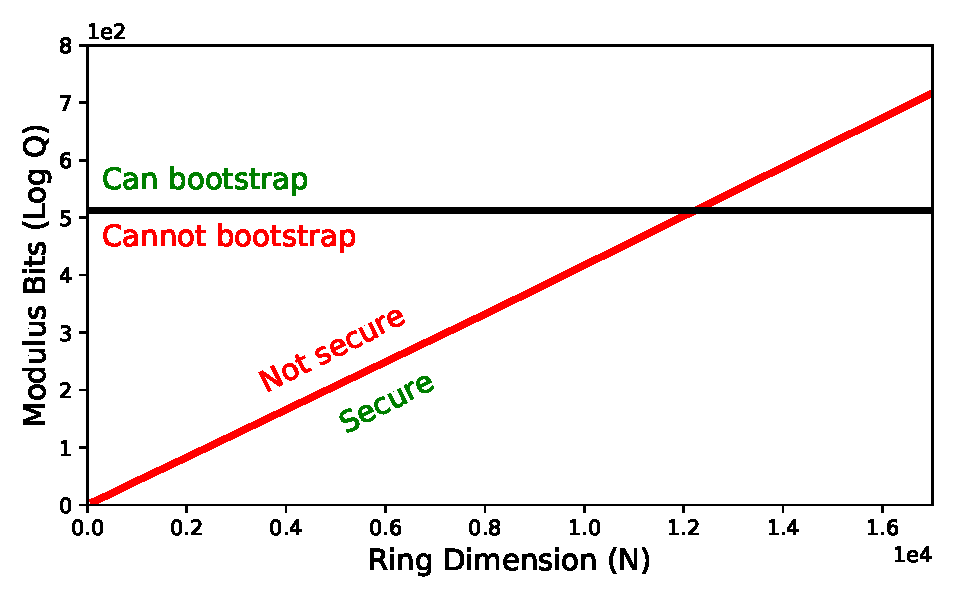
\includegraphics[width=0.75\columnwidth]{plots/security.pdf}
    \caption{Trade-offs between FHE parameters. Parameter values above the
      red line are deemed insecure (i.e., correspond to a security parameter below $80$ bits). The
      parameter values below the black line do not allow for bootstrapping.}
    \label{fig:paramTradeoffs}
    \vspace{-0.03in}
    \end{center}
  \end{figure}
}

\newcommand{\figArch}{
  \begin{figure}[h]
        \begin{center}
     \includegraphics[width=\columnwidth]{figures/ag_arch.pdf}
     \vspace{-0.12in} % this negative vspace... adds space  (which is what I want)
     \caption{Overview of the \name architecture.}
     \vspace{0.025in} % leave bottoms flush
    \label{fig:arch}
  \end{center}
  \end{figure}
}

\newcommand{\figMultDataflow}{
  \begin{figure}[h]
        \begin{center}
     \includegraphics[width=0.99\columnwidth]{figures/ag_mult_dataflow.pdf}
    \caption{Example matrix-vector multiply using FHE.}
    \label{fig:MultDataflow}
    \vspace{-0.1in}
    \end{center}
  \end{figure}
}

\newcommand{\figOpBreakdown}{
    \begin{figure}[h]
    \begin{center}
        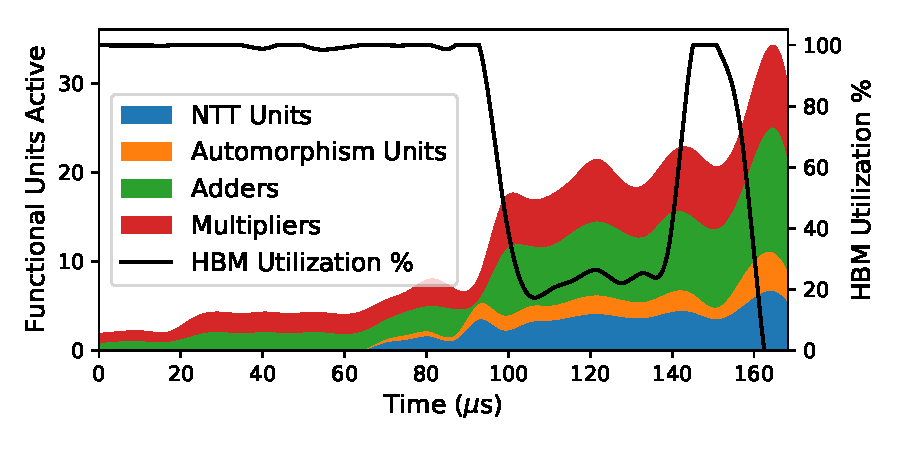
\includegraphics[width=0.7\columnwidth]{plots/lolaptwTimeplot.pdf}
        \caption{Functional unit and HBM utilization over time for the LoLa-MNIST PTW benchmark.}
        \label{fig:opBreakdown}
    \end{center}
    \end{figure}
}

\newcommand{\figCompilerOverview}{
  \begin{figure}[h]
        \begin{center}
     \includegraphics[width=\columnwidth]{figures/ag_compiler_overview.pdf}
    \caption{Overview of the \name compiler.}
    \label{fig:compilerOverview}
    %\vspace{-0.06in} %dsm: Shaves off a line, but looks bad
    \end{center}
  \end{figure}
}

\newcommand{\figautfu}{
\setlength{\columnsep}{7pt}
  \begin{figure}[h]
    \begin{center}
      \vspace{-0.8em}
     \includegraphics[width=0.25\columnwidth]{figures/ag_aut_fu.pdf}
    \caption{Automorphism unit.}
    \label{fig:aut_fu}
    \vspace{-0.4em} 
    \end{center}
  \end{figure}
}

\newcommand{\figAutomorphism}{
  \begin{figure}[h]
        \begin{center}
    \includegraphics[width=0.99\columnwidth]{figures/ag_automorphism.pdf}
    \caption{Applying $\sigma_3$ on a ciphertext of four 4-element chunks by using only permutations local to chunks.}
    \label{fig:automorphism}
    \end{center}
  \end{figure}
}

\newcommand{\figTranspose}{
  \begin{figure}[h]
    \centering
    \includegraphics[width=0.5\columnwidth]{figures/ag_transpose.pdf}
    \caption{The transpose unit.}
    \label{fig:transpose}
  \end{figure}
}

\newcommand{\figFourStepNTT}{
  \begin{figure}[h]
    \includegraphics[width=0.99\columnwidth]{figures/ag_four_step_ntt.pdf}
    \caption{Example of a four-step NTT datapath that uses 4-point NTTs to implement 16-point NTTs.}
    \label{fig:fourStepNTT}
    \vspace{1em}
  \end{figure}
}

\newcommand{\figQuadrantSwap}{
  \begin{figure}[h]
    \centering
    \includegraphics[width=0.75\columnwidth]{figures/ag_quadrant_swap.pdf}
    \caption{Transpose unit (right) and its component quadrant-swap unit (left).}
    \label{fig:quadrantSwap}
    \vspace{0.1in}
  \end{figure}
}

\newcommand{\figOverview}{
  \begin{figure}[h]
    \centering
    \vspace{-0.11in}
    \includegraphics[width=.8\columnwidth]{figures/ag_overview.pdf}
    \caption{FHE allows a user to securely offload computation to an untrusted server.}
    %old: \caption{Workflow showing how FHE is used to securely offload computation to an untrusted server.}
    \label{fig:overview}
    \vspace{0.2cm}
  \end{figure}
}

\newcommand{\figFUSweep}{
  \begin{figure}[h]
        \begin{center}
     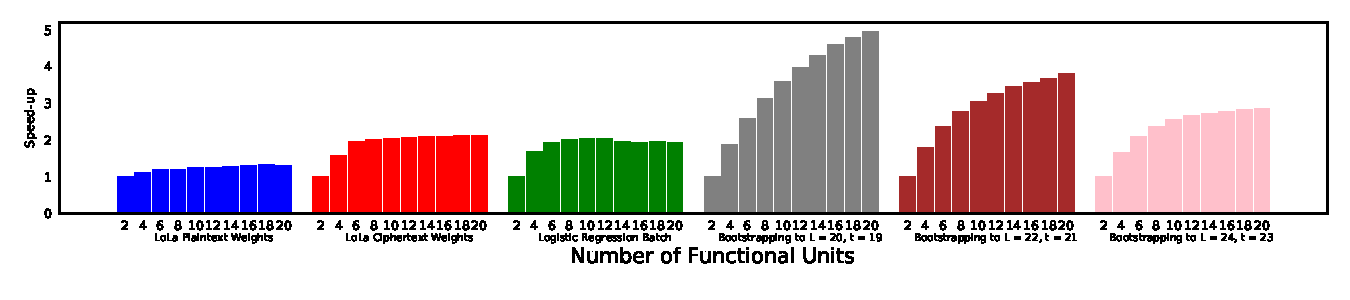
\includegraphics[width=\columnwidth]{plots/sweepFUs.pdf}
    \caption{Performance of our benchmarks with varying number of functional unit clusters.}
    \label{fig:sweepFUs}
    \vspace{-0.03in}
    \end{center}
  \end{figure}
}

\newcommand{\figBWSweep}{
  \begin{figure}[h]
        \begin{center}
     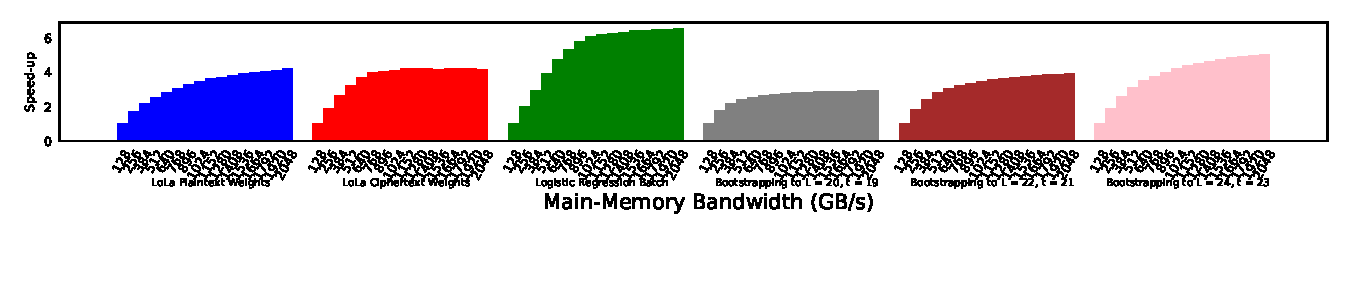
\includegraphics[width=\columnwidth]{plots/sweepBW.pdf}
    \caption{Performance of our benchmarks across various main memory bandwidths.}
    \label{fig:sweepBW}
    \vspace{-0.03in}
    \end{center}
  \end{figure}
}

\newcommand{\figDataMovement}{
\begin{figure}
  \centering
  \subfloat[]{
    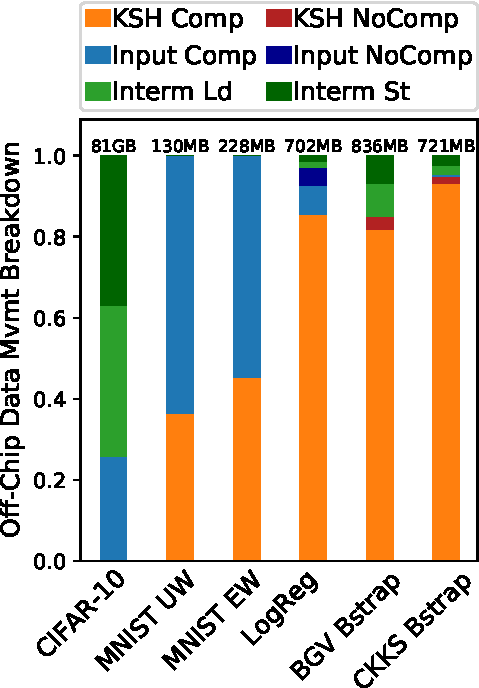
\includegraphics[width=0.4\linewidth]{plots/dataMovement.pdf}
    \label{fig:dataMovement}
  }
  \subfloat[]{
    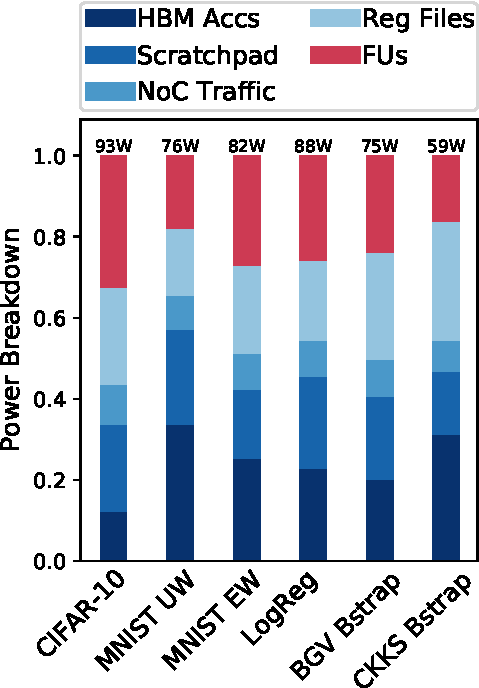
\includegraphics[width=0.4\linewidth]{plots/power.pdf}
    \label{fig:power}
  }
  \caption{Per-benchmark breakdowns of \textbf{(a)} data movement and \textbf{(b)} average power for \name.}
  %\vspace{0.1in}
\end{figure}
}

\newcommand{\figConfigs}{
    % \setlength{\columnsep}{7pt}
  \begin{figure}[h]
    % \vspace{-0.55in}
    \begin{center}
     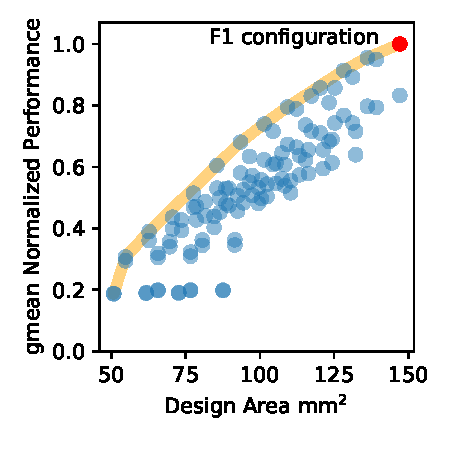
\includegraphics[width=0.45\columnwidth]{plots/configs.pdf}
    % \vspace{-0.26in}
    \caption{Performance vs. area across \name configurations.}
    \label{fig:pareto}
    % \vspace{-18pt}
    % \hspace{-0.03in}
    \end{center}
  \end{figure}
}

\newcommand{\figScratchpadSweep}{
  \begin{figure}[h]
        \begin{center}
     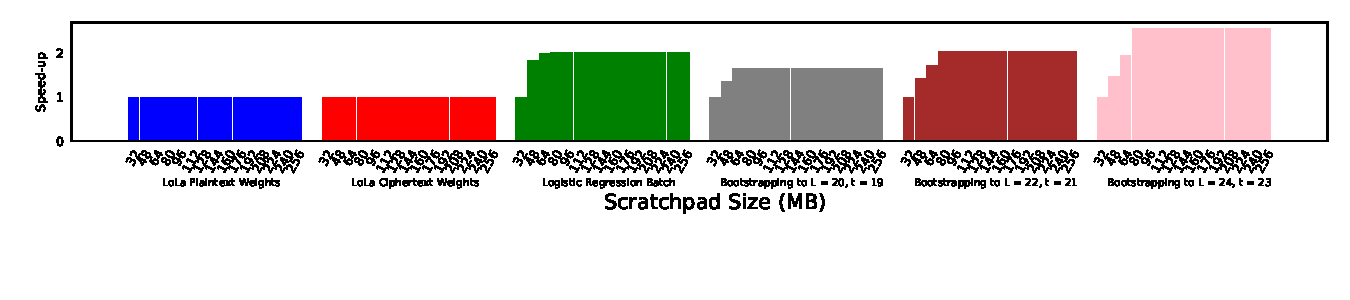
\includegraphics[width=\columnwidth]{plots/sweepScratchpad.pdf}
    \caption{Performance of our benchmarks across various scratchpad sizes.}
    \label{fig:sweepScratchpad}
    \vspace{-0.03in}
    \end{center}
  \end{figure}
}

\newcommand{\tblGF}{
  \begin{table}[h]
    \begin{center}
      \begin{footnotesize}
        \begin{tabular}{lrrr}
          \toprule
          Component & Area [mm$^2$] & TDP [W] \\
          \midrule
          NTT FU & 2.27 & 4.80  \\
          Automorphism FU & 0.58 & 0.99  \\
          %Transpose & 0.28 & \tmp{???} & - \\
          Multiply FU & 0.25 & 0.60  \\
          Add FU & 0.03 & 0.05  \\
          Vector RegFile (512\,KB) & 0.56 & 1.67 \\
          \textbf{Compute cluster} & 3.97 & 8.75 \\
          (NTT, Aut, 2$\times$ Mul, 2$\times$ Add, RF) & & \\
          \textbf{Total compute} (16 clusters) &  \textbf{63.52} & \textbf{140} \\
          \midrule
          Scratchpad (16$\times$4\,MB banks) & 48.09 & 20.35 \\
          3$\times$NoC (16$\times$16 512\,B bit-sliced~\cite{passas:tocaid12:crossbar}) & 10.02 & 19.65 \\
          Memory interface (2$\times$HBM2 PHYs) & 29.8 & 0.45 \\
          \textbf{Total memory system} &  \textbf{87.91} & \textbf{40.45} \\
          \midrule
          \textbf{Total \name} &  \textbf{151.43} & \textbf{180.45} \\
          \bottomrule
        \end{tabular}
      \end{footnotesize}
    \end{center}
    \vspace{-0.08in}
    \caption{Area and Thermal Design Power (TDP) of \name, and breakdown by component.}
    \label{tbl:GF12}
    \vspace{-0.1in}
  \end{table}
}


\newcommand{\tblNomenclature}{
   \begin{table}[h]
     \begin{footnotesize}
        \begin{center}
           \begin{tabular}{ll}
              \toprule
              \textbf{Param} & \textbf{Definition} \\
              \midrule
               \multicolumn{2}{c}{FHE Parameters} \\
              \midrule
              $N$ & Number of vector elements / polynomial coefficients \\
              $Q$ & Ciphertext modulus \\
              $t$ & Plaintext modulus \\
              \midrule
               \multicolumn{2}{c}{Architecture Parameters} \\
              \midrule
              $L$ & Number of RNS polynomials per ciphertext polynomial \\
              $q_i$ & The $i$-th RNS modulus ($Q = q_0q_1...q_{L-1}$) \\
              $E$ & Number of vector lanes \\
              $V$ & Vector operation initiation interval ($V = N/E$) \\ % dsm: Chimes? I don't know of a good nomenclature for this...
              \bottomrule
           \end{tabular}
           \label{tbl:nomenclature}
        \end{center}
        \caption{Nomenclature of key parameters in this paper.}
     \end{footnotesize}
   \end{table}
}

\newcommand{\tblModMult}{
  \begin{table}[h]
    \begin{footnotesize}
      \begin{center}
        \begin{tabular}{lrrr}
          \toprule
          Multiplier & Area [$\mu$m$^2$] & Power [mW] & Delay [ps] \\
          \midrule
          Barrett & $5,271$ & $18.4$ & 1,317 \\
          Montgomery & $2,916$ & $9.2$ & 1,040 \\
          NTT-friendly & $2,165$ & $5.36$ & 1,000 \\ % assumes q = 2^11m+1
          \midrule
          \textbf{FHE-friendly (ours)} & $1,817$ & $4.1$ & 1,000 \\
          \bottomrule
        \end{tabular}
        \vspace{0.02in}
        \caption{Area, power, and delay of modular multipliers.}
        \label{tbl:modMult}
      \end{center}
    \end{footnotesize}
    \vspace{-0.18in}
  \end{table}
}

\newcommand{\x}{$\times$}


\newcommand{\tblMicrobenchmark}{
  \begin{table}[t]
      % \vspace{-0pt}
      \begin{center}
      \resizebox{\columnwidth}{!}{%
      \begin{tabular}{l|rrr|rrr|rrr}
        \toprule
        & \multicolumn{3}{c|}{$N = 2^{12}$, $\log Q = 109$} &
        \multicolumn{3}{c|}{$N = 2^{13}$, $\log Q = 218$} &
        \multicolumn{3}{c}{$N = 2^{14}$, $\log Q = 438$} \\
        
        & \textbf{\name} & vs.\ CPU & vs.\ HEAX$_\sigma$ & \textbf{\name} & vs.\ CPU & vs.\ HEAX$_\sigma$ & \textbf{\name} & vs.\ CPU & vs.\ HEAX$_\sigma$\\

        \midrule

        % --- NTT

        % N=2**12, logQ = 109
        NTT
        &\textbf{12.8} % our
        &17,148$\times$ % CPU
        &1,600$\times$ % HEAX

        % N=2**13, logQ = 218
        &\textbf{44.8} % our
        &10,736$\times$ % CPU
        &1,733$\times$ % HEAX

        % N=2**14, logQ = 438
        &\textbf{179.2} % our
        &8,838$\times$ % CPU
        &1,866$\times$ % HEAX
        \\
        % --- Automorph. w/out k-s
        
        % N=2**12, logQ = 109
        Automorphism 
        &\textbf{12.8} % our
        &7,364$\times$ % CPU
        &440$\times$ % HEAX

        % N=2**13, logQ = 218   
        &\textbf{44.8} % our
        &8,250$\times$ % CPU
        &426$\times$ % HEAX

        % N=2**14, logQ = 438
        &\textbf{179.2} % our
        &16,957$\times$ % CPU
        &430$\times$ % HEAX
        \\

        \midrule

        % --- Ctxt-Ctxt Mult.

        % N=2**12, logQ = 109    
        Homomorphic multiply
        &\textbf{60} % our - % 60 MULS * 32 * 1/(32) = 60 cycles
        &48,640$\times$ % CPU
        &172$\times$ % HEAX

        % N=2**13, logQ = 218
        &\textbf{300} % our
        &27,069$\times$ % CPU
        &148$\times$ % HEAX

        % N=2**14, logQ = 438
        &\textbf{2,000} % our
        &14,396$\times$ % CPU
        &190$\times$ % HEAX
        \\

        % --- Automorph. w/ k-s

        % N=2**12, logQ = 109    
        Homomorphic permutation
        &\textbf{40} % our
        &17,488$\times$ % CPU
        &256$\times$ % HEAX

        % N=2**13, logQ = 218
        &\textbf{224} % our
        &10,814$\times$ % CPU
        &198$\times$ % HEAX

        % N=2**14, logQ = 438
        &\textbf{1,680} % our
        &6,421$\times$ % CPU
        &227$\times$ % HEAX
        \\
        
        \bottomrule
      \end{tabular}
      }
      %}
      \end{center}
      %\vspace{-5pt}
      \caption{Performance on microbenchmarks: \name's \textbf{reciprocal throughput, in nanoseconds per ciphertext operation} (lower is better) and speedups over CPU and HEAX$_\sigma$ (HEAX augmented with scalar automorphism units) (higher is better).}
      \label{tbl:microbenchmark}
      %\vspace{-3pt} % dsm: Leaves flush with other pages
  \end{table}
    % dsm: Now explained in text
    %\footnotetext[2]{We assume an SRAM array is used to perform an automorphism via random reads because HEAX does not report how they implement automorphisms.}
    %     \footnotetext[3]{We assume throughput is bottleneck on either the automorphism or keyswitching throughput, whichever is smaller.}
}


\newcommand{\tblBenchmark}{
  \begin{table}[t]
    \begin{footnotesize}
      \begin{center}
      \begin{tabular}{lrrr}
        \toprule
        Execution time (ms) on & CPU & \name & Speedup \\
        
        \midrule
        LoLa-CIFAR Unencryp. Wghts. & $1.2\times10^6$ & \textbf{241} & $5,011$\x \\
        LoLa-MNIST Unencryp. Wghts. & $2,960$ & \textbf{0.17} & $17,412$\x \\
        LoLa-MNIST Encryp. Wghts. & $5,431$ & \textbf{0.36} & $15,086$\x \\
        Logistic Regression & $8,300$ & \textbf{1.15} & $7,217$\x \\
        BGV Bootstrapping & ---\footnotemark[2] & \textbf{1.8} & ---\footnotemark[2] \\  % L=24
        CKKS Bootstrapping & $1,554$ & \textbf{1.3} & $1,195$\x \\    % L=24
        \midrule

        \textbf{gmean speedup} &&& 6,471\x \\
        % CKKS Bootstrapping $L=22$ & $1456$ & \textbf{2.2} & $662$\x \\
        % CKKS Bootstrapping $L=20$ & $1314$ & \textbf{1.9} & $692$\x \\
        \bottomrule
      \end{tabular}
   \end{center}
    \vspace{-8pt}
      \hfill\footnotemark[1]{LoLa's release did not include MNIST with encrypted weights, so we reimplemented it in HELib.}\quad\mbox{} \\
      \hfill\footnotemark[2]{BGV bootstrapping in HELib crashes for this input, and we could not find an alternative implementation or fix HELib. We expect \name's speedup to be at least 3,000$\times$}.\quad\mbox{}
    \end{footnotesize}
    \vspace{4pt}
      \caption{Performance of \name and CPU on full FHE benchmarks: execution times in milliseconds
      and \name's speedup.}      
      \label{tbl:benchmark}
      \vspace{-6pt}
  \end{table}
}

\newcommand{\tblPrimitiveOps}{
  \begin{table}[h]
    \begin{footnotesize}
      \begin{center}
        \caption{Operations in BGV \cite{}, CKKS \cite{}, and GSW \cite{} schemes and their constituent
        \textit{primitive operations}, which \name FUs acelerate. BGV and CKKS use very similar FHE operations
        and differ mainly in encryption/decryption.}
        \begin{tabular}{l|rr}
          \toprule
          & \multicolumn{2}{c}{\textbf{Required primitive operations}} \\
          \textbf{Operation} & \textbf{BGV/CKKS} & \textbf{GSW} \\
          \midrule
          Ciphertext add & add & add \\
          Ciphertext mult & NTT, mult & NTT, mult, add \\
          Key switching/relin & NTT, mult, add & N/A \\
          Mod switching & NTT, reduce, add & NTT, reduce, add \\
          Bootstrapping & automorphism, all ops & automorphism, all ops \\
          \bottomrule
        \end{tabular}
        \label{tbl:primitiveOps}
      \end{center}
    \end{footnotesize}
  \end{table}
}

\newcommand{\cipher}{\textsf{Ciphertext}}
\newcommand{\plain}{\textsf{Plaintext Vector}}
\newcommand{\scalar}{\textsf{Plaintext Scalar}}

\newcommand{\tblDSLOps}{
  \begin{table}[h]
    \begin{footnotesize}
      \begin{center}
        \caption{Supported FHE Operations and Types}
        \begin{tabular}{l|r}
            \textbf{Operation} & \textbf{Type}\\
            \midrule
            \textsf{Mul} & $\cipher \times \cipher \rightarrow \cipher$ \\
            \textsf{MulPlaintext} & $\cipher \times \plain \rightarrow \cipher$ \\
            \textsf{MulScalar} & $\cipher \times \scalar \rightarrow \cipher$ \\
            \textsf{Add} & $\cipher \times \cipher \rightarrow \cipher$ \\
            \textsf{AddPlaintext} & $\cipher \times \plain \rightarrow \cipher$ \\
            \textsf{AddScalar} & $\cipher \times \scalar \rightarrow \cipher$ \\
            \textsf{Rotate} & $\cipher \times \scalar \rightarrow \cipher$ \\
            \textsf{ModDown} & $\cipher \times \scalar \rightarrow \cipher$ \\
        \end{tabular}
      \end{center}
    \end{footnotesize}
  \end{table}
}


\newcommand{\tblSensitivity}{
  \begin{table}[h]
    \begin{footnotesize}
      \begin{center}
        \begin{tabular}{lrrr}
            \toprule
            Benchmark & LT NTT & LT Aut & CSR \\
            \midrule
            LoLa-CIFAR Unencryp. Wghts. & 3.5\x & 12.1\x & ---\footnotemark[1] \\
            LoLa-MNIST Unencryp. Wghts. & 5.0\x & 4.2\x & 1.1\x \\
            LoLa-MNIST Encryp. Wghts. & 5.1\x & 11.9\x & 7.5\x \\
            Logistic Regression & 1.7\x & 2.3\x & 11.7\x \\
            BGV Bootstrapping & 1.6\x & 1.1\x & 5.4\x \\
            CKKS Bootstrapping & 1.1\x & 1.2\x & 2.7\x \\
            \midrule
            \textbf{gmean speedup} & 2.5\x & 5.5\x & 4.2\x \\
            \bottomrule
        \end{tabular}
      \end{center}
      \vspace{-8pt}
      \hfill\footnotemark[1]{CSR is intractable for this benchmark.}\quad\mbox{}
    \end{footnotesize}
    \vspace{4pt}
        \caption{Speedups of \name over alternate configurations: %without our contributions:
          LT NTT/Aut = Low-throughput NTT/Automorphism FUs; CSR = Code Scheduling to minimize Register Usage \cite{goodman:ics1988:code}.}
        \label{tbl:sensitivity}
    \vspace{-2pt}
  \end{table}
}

\newcommand{\C}{\textsf{Scalar}}
\newcommand{\V}{\textsf{Vector}}
\newcommand{\q}{\textsf{Modulus}}

\newcommand{\tblISA}{
  \begin{table}[h]
  \begin{footnotesize}
  \begin{center}
  \caption{\name ISA}
  \begin{tabular}{lr}
  \toprule
  Instruction & Type \\
  \midrule
  \texttt{ADD} & $\V \times \V \times \q \rightarrow \V$ \\
  \texttt{ADD\_SCALAR} & $\V \times \C \times \q \rightarrow \V$ \\
  \texttt{MUL} & $\V \times \V \times \q \rightarrow \V$ \\
  \texttt{MUL\_SCALAR} & $\V \times \C \times \q \rightarrow \V$ \\
  \texttt{NTT} & $\V \times \q \rightarrow \V$ \\
  \texttt{INTT} & $\V \times \q \rightarrow \V$ \\
  \texttt{AUTOMORPHISM} & $\V \times \C \rightarrow \V$ \\
  \end{tabular}
  \label{tbl:isa}
  \end{center}
  \end{footnotesize}
  \end{table}
}


%% This file is for producing a Doctoral Thesis proposal.  It should be fairly
%% self-explanatory.

% \documentclass{article}
% \begin{document}

% \bibliographystyle{plain}
% \pagestyle{empty}
% \markboth{{\sc thesis proposal}}{{\sc thesis proposal}}
\def\titone{Enabling Real-time Private DNN Inference Using}
\def\tittwo{Fully Homomorphic Encryption}
\def\author{Nikola Samardzic}
\def\addrone{70 Pacific St}
\def\addrtwo{Cambridge, MA 02131}

\def\degree{Master of Science}
%% Added \deptname for PhD proposals in other fields.
%% Krishna Sethuraman (1990)
\def\deptname{Electrical Engineering and Computer Science}
\def\laboratory{Computer Science and Artificial Intelligence Laboratory}

%\def\submissiondate{\today}
\def\submissiondate{\today}
\def\completiondate{May 2022}

\def\supervisor{Professor Daniel Sanchez}
\def\supertitleone{Associate Professor}
\def\supertitletwo{of Electrical Engineering and Computer Science}


%%%%%%%%%%%%%%%%%%%%%%%%%%%%%%%%%%%%%%%%%%%%%%%%%%%%%%%%%%%%%%%%%%%%%%%%%%%%
%%%%%%%%%% You Should Not Need To Modify Anything Below Here %%%%%%%%%%%%%%%
%%%%%%%%%%%%%%%%%%%%%%%%%%%%%%%%%%%%%%%%%%%%%%%%%%%%%%%%%%%%%%%%%%%%%%%%%%%%

%%%%%%%%%%%%%%%%%%%%%%%%%%%%%%%%%
%%% Cover Page - Author signs %%%
%%%%%%%%%%%%%%%%%%%%%%%%%%%%%%%%%
\thispagestyle{empty}

\begin{center}
{\normalsize \bf
   Massachusetts Institute of Technology
\\ Department of \deptname \\}
\vspace{.15in}
{\normalsize \bf
   Proposal for Thesis Research in Partial Fulfillment
\\ of the Requirements for the Degree of
\\ \degree \\}
\end{center}

\vspace{.15in}

\def\sig{{\small \sc (Signature of Author)}}

\noindent\begin{tabular}{llc}
{\small \sc Title:}         & \multicolumn{2}{l}{\titone} \\
			                & \multicolumn{2}{l}{\tittwo} \\
{\small \sc Submitted by:}
                            & \author  & \\
                            & \addrone & \\
                            & \addrtwo & \vspace{.1in}\\
%                             &          & \\

{\small \sc Signature of Author:} &  \multicolumn{2}{l}{\rule[-1ex]{8cm}{0.3pt} } \\
{\small \sc Date of Submission:}          & \multicolumn{2}{l}{\submissiondate} \\
\multicolumn{3}{l}{{\small \sc Expected Date of Completion:} \completiondate} \\
{\small \sc Laboratory:}                  & \multicolumn{2}{l}{\laboratory}
\end{tabular}


\vspace{0.4in}
\noindent{\bf \sc Brief Statement of the Problem:}

{\small Computing in public datacenters requires users to trust their chosen Cloud Service Provider with access to the data their computations require. 
Given the sensitive nature of certain types of data, this is often undesirable.
Fully Homomorphic Encryption (FHE) provides a cryptographically secure, though computationally expensive,
method of performing computations on encrypted data.
To make homomorphically encrypted computations perform sufficiently well to be practically usable, 
we propose a novel programmable VLIW vector architecture.
We also propose techniques to efficiently map FHE programs onto this architecture.
}
\vspace{0.4in}

\noindent{\bf \sc Supervision Agreement:}\\
\indent{\small
The program outlined in this proposal is adequate for a Master's thesis.  The supplies and facilities required are available, and I am willing to supervise the research and evaluate the thesis report.}

\begin{raggedleft}
\rule[-1ex]{9cm}{0.3pt}\\
\end{raggedleft}
\begin{raggedleft}
Daniel Sanchez, Assoc. Prof. of EECS\\
\end{raggedleft}



%          %%%%%%%%%%%%%%%%%%%%%%%%%%%%%
% \newpage %%% Supervision Agreement %%%
%          %%%%%%%%%%%%%%%%%%%%%%%%%%%%%
% 
% \begin{flushright}
%    Massachusetts Institute of Technology
% \\ Department of \deptname
% \\ Cambridge, Massachusetts 02139
% \end{flushright}
% 
% \underline{\bf Doctoral Thesis Supervision Agreement}
% 
% \vspace{.25in}
% \begin{tabular}{rl}
%    {\small \sc To:}   & Department Graduate Committee
% \\ {\small \sc From:} & \supervisor
% \end{tabular}
% 
% \vspace{.25in}
% The program outlined in the proposal:
% 
% \vspace{.25in}
% \begin{tabular}{rl}
%    {\small \sc Title:}  & \title
% \\ {\small \sc Author:} & \author
% \\ {\small \sc Date:}   & \submissiondate
% \end{tabular}
% 
% \vspace{.25in}
% is adequate for a Doctoral thesis.
% I believe that appropriate readers for this thesis would be:
% 
% \vspace{.25in}
% \begin{tabular}{rl}
%    {\small \sc Reader 1:} & \readerone
% \\ {\small \sc Reader 2:} & \readertwo
% %\\ {\small \sc Reader 3:} & \readerthree
% \end{tabular}
% 
% \vspace{.25in}
% Facilities and support for the research outlined in the proposal are available.
% I am willing to supervise the thesis and evaluate the thesis report.
% 
% \vspace{.25in}
% \begin{tabular}{crc}
%   \hspace{2in} & {\sc Signed:} & \\ \cline{3-3}
%                &               & {\small \sc \supertitleone} \\
%                &               & {\small \sc \supertitletwo} \\
%                &               &                             \\
%                & {\sc Date:}   & \\ \cline{3-3}
% \end{tabular}
% 
% \vspace{0in plus 1fill}
% 
% Comments: \\
% \begin{tabular}{c}
%   \hspace{6.25in} \\
%   \mbox{} \\ \cline{1-1} \mbox{} \\
%   \mbox{} \\ \cline{1-1} \mbox{} \\
%   \mbox{} \\ \cline{1-1} \mbox{} \\
% %  \mbox{} \\ \cline{1-1} \mbox{} \\
% %  \mbox{} \\ \cline{1-1} \mbox{} \\
% %  \mbox{} \\ \cline{1-1} \mbox{} \\
% \end{tabular}
% 
%           %%%%%%%%%%%%%%%%%%%%%%%%%%
% \newpage  %%% Reader I Agreement %%%
%           %%%%%%%%%%%%%%%%%%%%%%%%%%
% 
% \begin{flushright}
%    Massachusetts Institute of Technology
% \\ Department of \deptname
% \\ Cambridge, Massachusetts 02139
% \end{flushright}
% 
% \underline{\bf Doctoral Thesis Reader Agreement}
% 
% \vspace{.25in}
% \begin{tabular}{rl}
%    {\small \sc To:}   & Department Graduate Committee
% \\ {\small \sc From:} & \readerone
% \end{tabular}
% 
% \vspace{.25in}
% The program outlined in the proposal:
% 
% \vspace{.25in}
% \begin{tabular}{rl}
%    {\small \sc Title:}          & \title
% \\ {\small \sc Author:}         & \author
% \\ {\small \sc Date:}           & \submissiondate
% \\ {\small \sc Supervisor:}     & \supervisor
% \\ {\small \sc Other Reader:}   & \readertwo
% %\\ {\small \sc Other Reader:}   & \readerthree
% \end{tabular}
% 
% \vspace{.25in}
% is adequate for a Doctoral thesis.
% I am willing to aid in guiding the research
% and in evaluating the thesis report as a reader.
% 
% \vspace{.25in}
% \begin{tabular}{crc}
%   \hspace{2in} & {\sc Signed:} & \\ \cline{3-3}
%                &               & {\small \sc \readeronetitleone} \\
%                &               & {\small \sc \readeronetitletwo} \\
%                &               &                                 \\
%                & {\sc Date:}   & \\ \cline{3-3}
% \end{tabular}
% 
% \vspace{0in plus 1fill}
% 
% Comments: \\
% \begin{tabular}{c}
%   \hspace{6.25in} \\
%   \mbox{} \\ \cline{1-1} \mbox{} \\
%   \mbox{} \\ \cline{1-1} \mbox{} \\
%   \mbox{} \\ \cline{1-1} \mbox{} \\
%   \mbox{} \\ \cline{1-1} \mbox{} \\
%   \mbox{} \\ \cline{1-1} \mbox{} \\
%   \mbox{} \\ \cline{1-1} \mbox{} \\
% \end{tabular}
% 
% 
%           %%%%%%%%%%%%%%%%%%%%%%%%%%%
% \newpage  %%% Reader II Agreement %%%
%           %%%%%%%%%%%%%%%%%%%%%%%%%%%
% 
% 
% \begin{flushright}
%    Massachusetts Institute of Technology
% \\ Department of \deptname
% \\ Cambridge, Massachusetts 02139
% \end{flushright}
% 
% \underline{\bf Doctoral Thesis Reader Agreement}
% 
% \vspace{.25in}
% \begin{tabular}{rl}
%    {\small \sc To:}   & Department Graduate Committee
% \\ {\small \sc From:} & \readertwo
% \end{tabular}
% 
% \vspace{.25in}
% The program outlined in the proposal:
% 
% \vspace{.25in}
% \begin{tabular}{rl}
%    {\small \sc Title:}          & \title
% \\ {\small \sc Author:}         & \author
% \\ {\small \sc Date:}           & \submissiondate
% \\ {\small \sc Supervisor:}     & \supervisor
% \\ {\small \sc Other Reader:}   & \readerone
% %\\ {\small \sc Other Reader:}   & \readerthree
% \end{tabular}
% 
% \vspace{.25in}
% is adequate for a Doctoral thesis.
% I am willing to aid in guiding the research
% and in evaluating the thesis report as a reader.
% 
% \vspace{.25in}
% \begin{tabular}{crc}
%   \hspace{2in} & {\sc Signed:} & \\ \cline{3-3}
%                &               & {\small \sc \readertwotitleone} \\
%                &               & {\small \sc \readertwotitletwo} \\
%                &               &                                 \\
%                & {\sc Date:}   & \\ \cline{3-3}
% \end{tabular}
% 
% \vspace{0in plus 1fill}
% 
% Comments: \\
% \begin{tabular}{c}
%   \hspace{6.25in} \\
%   \mbox{} \\ \cline{1-1} \mbox{} \\
%   \mbox{} \\ \cline{1-1} \mbox{} \\
%   \mbox{} \\ \cline{1-1} \mbox{} \\
%   \mbox{} \\ \cline{1-1} \mbox{} \\
%   \mbox{} \\ \cline{1-1} \mbox{} \\
%   \mbox{} \\ \cline{1-1} \mbox{} \\
% \end{tabular}
% \newpage
%           %%%%%%%%%%%%%%%%%%%%%%%%%%%
% \newpage  %%% Reader III Agreement %%%
%           %%%%%%%%%%%%%%%%%%%%%%%%%%%
% 
% 
% \begin{flushright}
%    Massachusetts Institute of Technology
% \\ Department of \deptname
% \\ Cambridge, Massachusetts 02139
% \end{flushright}
% 
% \underline{\bf Doctoral Thesis Reader Agreement}
% 
% \vspace{.25in}
% \begin{tabular}{rl}
%    {\small \sc To:}   & Department Graduate Committee
% \\ {\small \sc From:} & \readerthree
% \end{tabular}
% 
% \vspace{.25in}
% The program outlined in the proposal:
% 
% \vspace{.25in}
% \begin{tabular}{rl}
%    {\small \sc Title:}          & \title
% \\ {\small \sc Author:}         & \author
% \\ {\small \sc Date:}           & \submissiondate
% \\ {\small \sc Supervisor:}     & \supervisor
% \\ {\small \sc Other Reader:}   & \readerone
% \\ {\small \sc Other Reader:}   & \readertwo
% \end{tabular}
% 
% \vspace{.25in}
% is adequate for a Doctoral thesis.
% I am willing to aid in guiding the research
% and in evaluating the thesis report as a reader.
% 
% \vspace{.25in}
% \begin{tabular}{crc}
%   \hspace{2in} & {\sc Signed:} & \\ \cline{3-3}
%                &               & {\small \sc \readerthreetitleone} \\
%                &               & {\small \sc \readerthreetitletwo} \\
%                &               &                                 \\
%                & {\sc Date:}   & \\ \cline{3-3}
% \end{tabular}
% 
% \vspace{0in plus 1fill}
% 
% Comments: \\
% \begin{tabular}{c}
%   \hspace{6.25in} \\
%   \mbox{} \\ \cline{1-1} \mbox{} \\
%   \mbox{} \\ \cline{1-1} \mbox{} \\
%   \mbox{} \\ \cline{1-1} \mbox{} \\
%   \mbox{} \\ \cline{1-1} \mbox{} \\
%   \mbox{} \\ \cline{1-1} \mbox{} \\
%   \mbox{} \\ \cline{1-1} \mbox{} \\
% \end{tabular}
% \newpage

% \end{document}
\cleardoublepage
% \thispagestyle{empty}
\setcounter{page}{1}

\section{Introduction}

\subsection{Fully Homomorphic Encryption}

A significant portion of computing workloads are now executed in the cloud.
However, executing a program in the cloud involves users to trust their chosen Cloud Service Provider (CSP)
with access to the data their computations require. Even if a user's trusted CSP is not maliciously inspecting their data,
the CSP is suceptible to being hacked by other actors who can now access user data.
For sensitive information such as health records or financial information, this risk might
be unacceptable.

Fully Homomorphic Encryption (FHE) provides a promising solution to this problem.
FHE systems provide a cryptographically secure method, though computationally expensive, to perform computations on
encrypted data \cite{gentry:stoc09:fhe, brakerski:itcs12:bgv, cheon:asiacrypt2017:ckks}.
Specifically, FHE allows for a ``server" to evaluate an arbitrary arithmetic
circuit of additions and mulitplications on encrypted inputs.
This means that the ``user", who provides the encrypted inputs and a set of public keys, 
does not need to trust the server with access to their data.

Writing an FHE program is quite different from writing a program in a standard
programming language like C++ or Python. 
FHE programs must be arithmetic \emph{circuits}, meaning that 
data dependent branches, and therefore loops, are impossible to express.
The intuitition behind this is that a program cannot branch on data it cannot
even decrypt. This means that not all standard ``plaintext" (unencrypted) programs
can be efficiently translated into FHE programs. Importantly, many numeric
programs including linear algebra, logistic regression, and neural networks
\emph{can} be written as arithmetic circuits 
\cite{halevi:acc14:algo-helib, han:iaai19:he-logreg, dowlin:icml16:cryptonets}.
These algorithms are also particularly appealing candidates for homomorphic
encryption because they are often run on sensitive data.

Unfortunately, all FHE programs have significant computational overheads 
over standard plaintext programs.
Several software libraries \cite{palisade, helib, seal}
implement state of the art FHE cryptosystems, but they all
suffer from several order-of-magnitude slowdowns over plaintext computations.
These massive slowdowns make running homomorphically encrypted programs
infeasible in practice.
Hardware acceleration seems like a promising approach to closing the
performance gap between FHE and plaintext computations.

\subsection{Prior Work}

To this end, several FPGA accelerators have been proposed, each showing
substantial speedups over CPU-based software implementations
\cite{riazi:asplos20:heax, roy:hpca19:he-fpga}.
However, these FPGA designs present several drawbacks. 
FPGAs cannot emulate all of the logic required to execute a full FHE program
simultaneously, and are therefore limited to accelerating only limited chunks
of the overall computation at once.
Additionally, an FPGA design must be tailored to a specfic FHE cryptosystem and
arithmetic circuit, leaving limited flexibility at runtime. 
Finally, FPGAs are very power hungry and have very limited clock speeds.

Furthermore, all existing accelerators fall short of performing
\emph{Fully} Homomorphic Encryption, and instead only implement
\emph{Somewhat} Homomorphic Encryption (SHE). The key difference is that
SHE circuits can only be of limited depth; a specific value cannot be the
result of more than a fixed number of operations, otherwise it will become
too noisy and therefore undecryptable. 
To turn a SHE scheme into a FHE scheme,
we need a \emph{bootstrapping} operation which ``resets" an encrypted value's
noise. Bootstrapping operations have been implemented in FHE software
libraries, but to our knowledge, no one has attempted to accelerate
bootstrapping in hardware. Supporting bootstrapping would allow an accelerator
to support more complex linear algebra computations, deeper neural networks,
and more training iterations for logistic regression.

\section{Proposal}

We propose a Very Long Instruction Word (VLIW) vector architecture targeting
the widely used BGV \cite{brakerski:itcs12:bgv} and CKKS \cite{cheon:asiacrypt2017:ckks}
FHE systems.

\subsection{Characteristics of Targeted FHE Schemes}

The following applies generally to all the cryptosystems we target.

Let $R = \mathbb{Z}[z]/(x^N+1)$. Our ciphertexts are stored as pairs of
polynomials in the quotient ring $R_q = R /qR$ where $q$ is the product of
32-bit primes $q_1, \dots, q_L$. We note that this introduces two parameters
to our ciphertext space: $N$ and $L$. $N$ is the degree of our polynomial, 
and therefore the number of coefficients we must store for each ciphertext.
$L$, by determining the number of 32-bit primes which make up the modulus,
controls the bit-width of the coefficients.

Each ciphertext encrypts a vector of $S$ many plaintext elements.
$S$, often referred to in the FHE literature as the number of ``SIMD-slots",
is picked between $1$ and $N$, and is fixed for all ciphertexts in a particular
computation. 
Homomorphically adding two ciphertexts $a, b$ will result in adding the
values stored in their respective SIMD-slots element-wise.
Homomorphically multiplying two ciphertexts $a, b$ will proceed analogously.
The values stored in SIMD-slots can be permuted by applying various
\emph{automorphisms} to a ciphertext. We can regard addition, multiplication,
and automorphisms as the building blocks of any homomorphically encrypted
program.

As we perform homomorphic operations, the resulting ciphertexts will accumulate
\emph{noise}. Once the noise exceeds a fixed threshold, a ciphertext becomes
undecipherable. Homomorphic multiplication adds significant noise, while both
automorphisms and homomorphic addition add minimal noise.
In order to avoid this happening, we can \emph{bootstrap} it to reset its noise.
Bootstrapping is a computationally expensive operation, and also an active area
of mathematical research.

Homomorphic addition is performed by adding the respective polynomials of the
two operand ciphertexts. Homomorphic multiplication is performed analogously,
but with polynomial mulitplication instead of addition. Automorphisms are
performed by applying a specific set of permutations to the ciphertext
coefficients. Importantly, both multiplication as well as automorphisms
require a ``key-switching" step after being completed to make the result
interoperable with other ciphertexts. This key-switching step involves
matrix-vector multiplication with a set of key-switching hints that are provided
as part of the public key.

Our proposed accelerator will target values of $N$ from $2^10$ to $2^14$ and
values of $L$ from 7 to 16. Fundamentally, $N$ impacts the security of our
encryption scheme, with higher values of $N$ resulting in more secure
encryption. $L$ decides the number of homomorphic operations we can do between
bootstrapping. Each $L$ can be thought of as a level, and performing a
homomorphic multiplication reduces a ciphertext's level by 1. A ciphertext must
be bootstrapped before its level decreases below $L_{min}$, which is the 
number of levels required to perform the boostrapping operation itself.

There are two mathematical optimizations, widely utilized in the existing
literature, which we will also be targeting. The first is using a 
Residue Number System to avoid wide bit arithmetic. Consider $L = 16$, in
this scenario, $q$ is a 512-bit prime, meaning that all coefficients must
also be 512-bits wide. Homomorphic addition, multiplication, and key-switching
would all require 512-bit wide adders and multipliers, which would be
area-inefficient given the quadratic overhead of these circuits.
Instead, using RNS, we can store each coefficient as an array of its residues
mod $q_1, \dots, q_L$. Each of these residues will be only 32-bits wide,
allowing us to use 32-bit multipliers and adders, and use the
Chinese Remainder Theorem (CRT) to reconstitute our original 512-bit wide
coefficients upon final decryption. The second optimization is applying a
type of Discrete Fourier Transform, known as a Number Theoretic Transform (NTT),
to all of our polynomials and operating on them in the NTT-domain. Doing so
transforms polynomial multiplications from the basic $O(n^2)$ method to a simple
$O(n)$ coefficient-wise multiplication. However, it does require the
introduction of custom functional units to perform NTTs at high
throughput.

\subsection{Architecture}

Our proposed architecture is based on two key observations about FHE programs.
The first is that FHE programs are completely static: as they lack any
branching behavior, the entire program dataflow is fixed. This means
that we can take advantage of VLIW scheduling techniques to statically
schedule programs at compile-time and avoid any sort of expensive dynamic
speculation systems. 
We are also able to use explicit data orchestration techniques, bringing
data to and from an on-chip scratchpad as needed.
The second observation is that FHE programs can be
implemented with relatively few different functional units: adders,
multipliers, NTT units, and automorphism (``shuffler") units.

Combining these two observations, we propose a vector VLIW processor with
explicit data orchestration. Our architecture will have the four types
of functional units required, with the exact number of each to be determined
over the course of our work. We will consider area vs. throughput tradeoffs
to decide how many of each functional unit we should incorporate.

The specific design and synthesis of each type of functional unit is being
studied by another member of our research group, and the results of this
will determine the architectural tradeoffs involved. 
We will also explore different types of memory (HBM vs. DDR) and their impact
on the overall performance our accelerator can achieve. 
Our initial estimates suggest that 128-wide vector units may work well for our
design, however, the vector width is subject to change as needed. The same goes
for our initial scratchpad size of 48MB.

\subsection{Workloads}

We will focus on accelerating existing programs optimized and designed for
FHE systems. Specifically, we will implementing a logistic regression
algorithm like the one described in \cite{han:iaai19:he-logreg} and neural
networks with plaintext weights like the ones described in 
\cite{dowlin:icml16:cryptonets}. We will also evaluate more basic FHE programs
such as matrix-vector multiply and bootstrapping.

Our accelerator design focuses on providing a flexible, programmable platform
for FHE acceleration, so we will not focus on a single specific cryptosystem
or set of initial parameters ($N, L$). Instead, we will perform a more complete
design space exploration, aiming to show that our proposed design is
general enough to accelerate different programs across
cryptosystems with different starting parameters.
For comparrison to existing FPGA-accelerators, we will also perform simpler
benchmarks featuring just additions and multiplications.

\subsection{Scheduling}

As mentioned, the extremely static nature of FHE programs allows for all
instruction and data scheduling to occur at compile-time. This requires
an effective scheduling algorithm to efficiently utilize the accelerator
resources. An effective scheduling algorithm is also essential to performing
a well-informed design-space exploration of our accelerator architecture.
Determining the resource requirements needed to run different programs requires
a detailed knowledge of how those particular programs would map to accelerator
designs with differing numbers of functional units, scratchpad sizes, and
memory subsystems.

To this end, a large focus of my research will be designing and implementing
an effective FHE scheduling algorithm. Our input programs will be described
as dataflow graphs, detailing the particular additions, mulitplications,
and automorphisms required to execute a given computation. We propose a
``scheduler frontend" which will take this dataflow graph expressed at a
ciphertext-level and lower it to a dataflow graph at a ``residue-polynomial"
level (polynomials of coefficients mod the same $q_i$).

This residue-polynomial level dataflow graph will then be passed through
a ``scheduler backend" which will also take a specific accelerator design
as an input, and add loads, stores, evictions, and instruction timings to the
inputted dataflow graph. When working correctly, the scheduler should produce
a near-optimal cycle-accurate schedule for specific dataflow graph on a
specific accelerator design.

Optimal scheduling is an NP-hard problem, so our scheduler will be focused
on robust heuristics as well as iterative improvement of a specific schedule.
It is interesting to note that given the completely static nature of this
computation, it is possible to evaluate Belady's Min algorithm for optimal
cache replacement. This algorithm is not possible in many more dynamic systems,
as it requires perfect foresight. We will investigate different instruction 
issuing heuristics to determine
efficient tradeoffs between increasing parallelism and maximizing the 
reuse of on-chip operands. Finally, memory bandwidth is sure to be a scarce
resource, regardless of whether we use HBM or a DDR-based system. Our proposed
scheduling algorithm will need to ensure that memory bandwidth is effectively
utilized to avoid our accelerator becoming hopelessly memory-bound.

Traditionally, VLIW systems have struggled with the tradeoff between maximizing
pipeline parallelism and code-footprint blowup. We believe that our system will
not inherently suffer from this problem, as the size of our operands is
significantly larger than single-word or double-word operands in existing VLIW
systems, and will therefore amortize an increased instruction footprint.
As part of our research, we will verify that this is indeed the case,
and if we find this assumption to be faulty, we will consider design
strategies to add loop control-flow to our programs and therefore
shrink code-size.

\subsection{Proposed Evaluation}

We will evaluate the performance of our designs in a simulated environment.
Our accelerator design tradeoffs will be informed by area estimates from
individually synthesized functional units. Using these area estimates,
we will use our proposed scheduling algorithm to sweep achievable
accelerator designs and produce cycle-accurate simulated performance results.
We will also verify that all schedules are correct and achievable.

Each of the workloads described earlier 
will be evaluated across a sweep of different
encryption parameters and input data sizes to ensure that our results are
representative of real FHE use-cases.


\section{Proposed Schedule}

\begin{table}[h]
\centering
\begin{tabular}{l p{0.7\textwidth}}
\toprule[1.5pt]
Time & Work Description \\
\hline
Summer 2020 & Gain a functional understanding of FHE systems, algorithms, and
 their implementations\\
Nov 2020 & Begin implementing scheduling algorithm, understand heuristics and their tradeoffs. Create dataflow graph for logistic regression.\\
Dec 2020-Jan 2021 & Improve scheduling algorithm, investigate different accelerator designs, and implement dataflow graph for neural network. Additionally, understand the differences between BGV and CKKS dataflow graphs.\\
Feb-Mar 2021 & Complete scheduling algorithm, focusing specifically on register allocation and FHE bootstrapping.\\
Apr 2021 & Perform design space explorations using the completed scheduling algorithm.\\
May 2021 & Compile results, understand fair comparisons against prior work, and run further experiments.\\
\bottomrule[1.5pt]
\end{tabular}
\end{table}


\begin{singlespacing}
%\bibliographystyle{unsrt}
%\bibliographystyle{ieeetr}
\bibliographystyle{IEEEtranS} % order references by author name
\bibliography{refs,confs}
\end{singlespacing}

\end{document}

